\documentclass{article}
\usepackage {inputenc, fullpage, listings, amsmath, graphicx, xcolor, blkarray}


\parindent 0pt

\title{%
   CSc 226: Algorithms and Data Structures II (Spring 2022) \\
   \large Written Assignment 4\\
    Alex Holland V00}
    
\date{}

\begin{document}

\maketitle

{\bf Question 1}\\

Consider the graph from the lecture 17 slides:
\begin{center}
    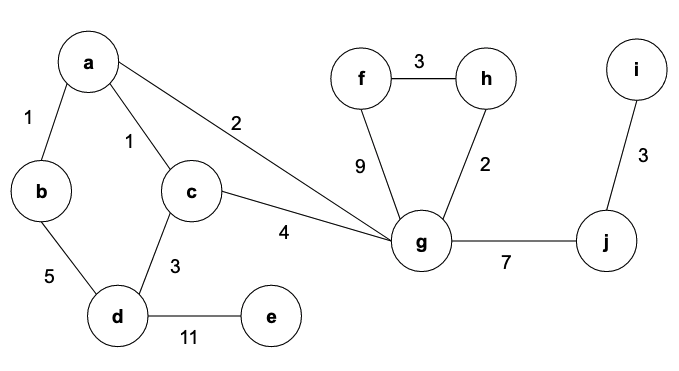
\includegraphics[width=0.75\textwidth]{1.png}
\end{center}

Each node pulled into the cloud is represented in \textcolor{blue}{blue}.\\
Distance values that have been updated are represented in \textcolor{red}{red}.\\
We will represent each step of the Dijkstra's algorithm as (Vertex, Distance value)\\

\smallskip
Initialization:\\
$(a, + \infty), (b, + \infty), (c, + \infty), (d, + \infty), (e, + \infty), (f, + \infty), (g, 0), (h, + \infty), (i, + \infty), (j, + \infty)$\\

Distance values at vertex g:\\
$\textcolor{red}{(a, 2)}, (b, + \infty), \textcolor{red}{(c, 4)}, (d, + \infty), (e, + \infty), \textcolor{red}{(f, 9)}, \textcolor{blue}{(g, 0)}, \textcolor{red}{(h, 2)}, (i, + \infty), \textcolor{red}{(j, 7)}$\\

Distance values at vertex a:\\
$\textcolor{blue}{(a, 2)}, \textcolor{red}{(b, 3)}, \textcolor{red}{(c, 3)}, (d, + \infty), (e, + \infty), (f, 9), \textcolor{blue}{(g, 0)}, (h, 2), (i, + \infty), (j, 7)$\\

Distance values at vertex h:\\
$\textcolor{blue}{(a, 2)}, (b, 3), (c, 3), (d, + \infty), (e, + \infty), \textcolor{red}{(f, 5)}, \textcolor{blue}{(g, 0)}, \textcolor{blue}{(h, 2)}, (i, + \infty), (j, 7)$\\

Distance values at vertex b:\\
$\textcolor{blue}{(a, 2)}, \textcolor{blue}{(b, 3)}, (c, 3), \textcolor{red}{(d, 7)}, (e, + \infty), (f, 5), \textcolor{blue}{(g, 0)}, \textcolor{blue}{(h, 2)}, (i, + \infty), (j, 7)$\\

Distance values at vertex c:\\
$\textcolor{blue}{(a, 2)}, \textcolor{blue}{(b, 3)}, \textcolor{blue}{(c, 3)}, \textcolor{red}{(d, 6)}, (e, + \infty), (f, 5), \textcolor{blue}{(g, 0)}, \textcolor{blue}{(h, 2)}, (i, + \infty), (j, 7)$\\

Distance values at vertex f:\\
$\textcolor{blue}{(a, 2)}, \textcolor{blue}{(b, 3)}, \textcolor{blue}{(c, 3)}, (d, 6), (e, + \infty), \textcolor{blue}{(f, 5)}, \textcolor{blue}{(g, 0)}, \textcolor{blue}{(h, 2)}, (i, + \infty), (j, 7)$\\

Distance values at vertex d:\\
$\textcolor{blue}{(a, 2)}, \textcolor{blue}{(b, 3)}, \textcolor{blue}{(c, 3)}, \textcolor{blue}{(d, 6)}, \textcolor{red}{(e, 17)}, \textcolor{blue}{(f, 5)}, \textcolor{blue}{(g, 0)}, \textcolor{blue}{(h, 2)}, (i, + \infty), (j, 7)$\\

Distance values at vertex j:\\
$\textcolor{blue}{(a, 2)}, \textcolor{blue}{(b, 3)}, \textcolor{blue}{(c, 3)}, \textcolor{blue}{(d, 6)}, (e, 17), \textcolor{blue}{(f, 5)}, \textcolor{blue}{(g, 0)}, \textcolor{blue}{(h, 2)}, \textcolor{red}{(i, 10)}), (j, 7)$\\

Distance values at vertex i:\\
$\textcolor{blue}{(a, 2)}, \textcolor{blue}{(b, 3)}, \textcolor{blue}{(c, 3)}, \textcolor{blue}{(d, 6)}, (e, 17), \textcolor{blue}{(f, 5)}, \textcolor{blue}{(g, 0)}, \textcolor{blue}{(h, 2)}, \textcolor{blue}{(i, 10)}), (j, 7)$\\

Distance values at vertex e:\\
$\textcolor{blue}{(a, 2)}, \textcolor{blue}{(b, 3)}, \textcolor{blue}{(c, 3)}, \textcolor{blue}{(d, 6)}, \textcolor{blue}{(e, 17)}, \textcolor{blue}{(f, 5)}, \textcolor{blue}{(g, 0)}, \textcolor{blue}{(h, 2)}, \textcolor{blue}{(i, 10)}, \textcolor{blue}{(j, 7)}$\\

Now all nodes have been pulled into the cloud and we have found the single source shortest path.

\bigskip
{\bf Question 2}\\
Consider the graph from the Lecture 18 slides-BF:
\begin{center}
    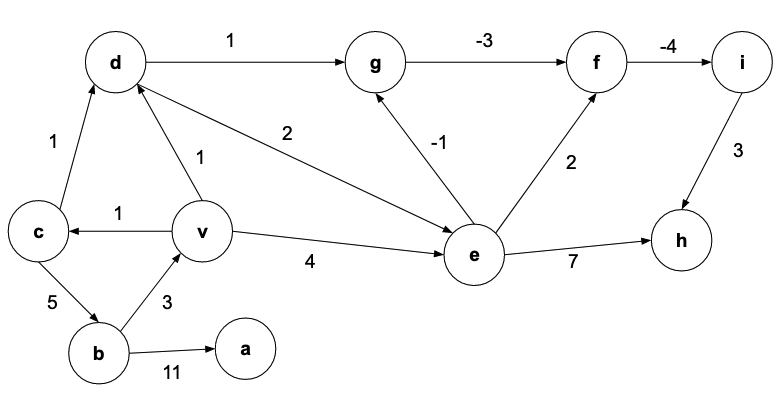
\includegraphics[width=0.75\textwidth]{2.png}
\end{center}

The following outbound edges are in lexicographical order:
\begin{center}
\begin{tabular}{||c c c c c c c c c c c c c c c||} 
 \hline
 b-a & b-v & c-b & c-d & d-e & d-g & e-f & e-g & e-h & f-i & g-f & i-h & v-c & v-d & v-e\\ [0.5ex] 
 \hline\hline
 11 & 3 & 5 & 1 & 2 & 1 & 2 & -1 & 7 & -4 & -3 & 3 & 1 & 1 & 4\\ 
 \hline
\end{tabular}
\end{center}

Initial values at vertex b:\\
$(a, + \infty), (b, 0), (c, + \infty), (d, + \infty), (e, + \infty), (f, + \infty), (g, + \infty), (h, + \infty), (i, + \infty), (v, + \infty)$\\

The number of iterations required by Bellman-Ford's algorithm is $n-1$, so we require $10-1=9$ iterations.\\

Sequence of changes during the 1st iteration:
\begin{enumerate}
    \item Node $a$ is affected, and its $D$ value has been updated to 11. 
    \item Node $v$ is affected, and its $D$ value has been updated to 3. 
    \item Node $c$ is affected, and its $D$ value has been updated to 4.   
    \item Node $d$ is affected, and its $D$ value has been updated to 4.
    \item Node $e$ is affected, and its $D$ value has been updated to 7.
\end{enumerate}

Sequence of changes during the 2nd iteration:
\begin{enumerate}
    \item Node $e$ is affected, and its $D$ value has been updated to 6.
    \item Node $g$ is affected, and its $D$ value has been updated to 5.
    \item Node $f$ is affected, and its $D$ value has been updated to 8.
    \item Node $h$ is affected, and its $D$ value has been updated to 13.
    \item Node $i$ is affected, and its $D$ value has been updated to 4.
    \item Node $f$ is affected, and its $D$ value has been updated to 2.
    \item Node $h$ is affected, and its $D$ value has been updated to 7.
\end{enumerate}

Sequence of changes during the 3rd iteration:
\begin{enumerate}
    \item Node $i$ is affected, and its $D$ value has been updated to -2.
    \item Node $h$ is affected, and its $D$ value has been updated to 1.
\end{enumerate}

The Bellman-Ford algorithm was determined to have 9 iterations, however no modifications to the nodes occur after the 3rd iteration. Thus the nodes and there D values at the end of the Bellman-Ford's algorithm is:\\

$(a, 11), (b, 0), (c, 4), (d, 4), (e, 6), (f, 2), (g, 5), (h, 1), (i, -2), (v, 3)$

\bigskip
{\bf Question 3}\\
Consider the graph:
\begin{center}
    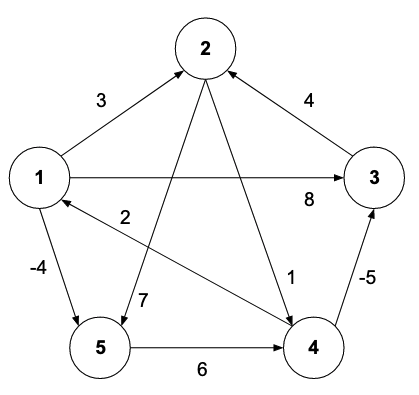
\includegraphics[width=0.4\textwidth]{3.png}
\end{center}

To determine the shortest path between all pairs of vertices using Floyd-Warshall algorithm. Consider the matrices A of dimension $n \times n$ where $n$ is the number of vertices. Values highlighted in \textcolor{red}{red} represent $D$ values that have been changed.

\begin{equation*}
A^0=
    \begin{blockarray}{c c c c c c}
        1 & 2 & 3 & 4 & 5 \\
        \begin{block}{(c c c c c)c}
            0 & 3 & 8 & +\infty & -4 & 1 \\
            +\infty & 0 & +\infty & 1 & 7 & 2 \\
            +\infty & 4 & 0 & +\infty & +\infty & 3 \\
            2 & +\infty & -5 & 0 & +\infty & 4 \\
            +\infty & +\infty & +\infty & 6 & 0 & 5 \\
        \end{block}
    \end{blockarray}
\end{equation*}

\begin{equation*}
A^1=
    \begin{blockarray}{c c c c c c}
        1 & 2 & 3 & 4 & 5 \\
        \begin{block}{(c c c c c)c}
            0 & 3 & 8 & +\infty & -4 & 1 \\
            +\infty & 0 & +\infty & 1 & 7 & 2 \\
            +\infty & 4 & 0 & +\infty & +\infty & 3 \\
            2 & \textcolor{red}{5} & -5 & 0 & \textcolor{red}{-2} & 4 \\
            +\infty & +\infty & +\infty & 6 & 0 & 5 \\
        \end{block}
    \end{blockarray}
\end{equation*}

\begin{equation*}
A^2=
    \begin{blockarray}{c c c c c c}
        1 & 2 & 3 & 4 & 5 \\
        \begin{block}{(c c c c c)c}
            0 & 3 & 8 & \textcolor{red}{4} & -4 & 1 \\
            +\infty & 0 & +\infty & 1 & 7 & 2 \\
            +\infty & 4 & 0 & \textcolor{red}{5} & \textcolor{red}{11} & 3 \\
            2 & 5 & -5 & 0 & -2 & 4 \\
            +\infty & +\infty & +\infty & 6 & 0 & 5 \\
        \end{block}
    \end{blockarray}
\end{equation*}

\begin{equation*}
A^3=
    \begin{blockarray}{c c c c c c}
        1 & 2 & 3 & 4 & 5 \\
        \begin{block}{(c c c c c)c}
            0 & 3 & 8 & 4 & -4 & 1 \\
            +\infty & 0 & +\infty & 1 & 7 & 2 \\
            +\infty & 4 & 0 & 5 & 11 & 3 \\
            2 & \textcolor{red}{-1} & -5 & 0 & -2 & 4 \\
            +\infty & +\infty & +\infty & 6 & 0 & 5 \\
        \end{block}
    \end{blockarray}
\end{equation*}

\begin{equation*}
A^4=
    \begin{blockarray}{c c c c c c}
        1 & 2 & 3 & 4 & 5 \\
        \begin{block}{(c c c c c)c}
            0 & 3 & \textcolor{red}{-1} & 4 & -4 & 1 \\
            \textcolor{red}{3} & 0 & \textcolor{red}{-4} & 1 & \textcolor{red}{-1} & 2 \\
            \textcolor{red}{7} & 4 & 0 & 5 & \textcolor{red}{3} & 3 \\
            2 & -1 & -5 & 0 & -2 & 4 \\
            \textcolor{red}{8} & \textcolor{red}{5} & \textcolor{red}{1} & 6 & 0 & 5 \\
        \end{block}
    \end{blockarray}
\end{equation*}

\begin{equation*}
A^5=
    \begin{blockarray}{c c c c c c}
        1 & 2 & 3 & 4 & 5 \\
        \begin{block}{(c c c c c)c}
            0 & \textcolor{red}{1} & \textcolor{red}{-3} & \textcolor{red}{2} & -4 & 1 \\
            3 & 0 & -4 & 1 & -1 & 2 \\
            7 & 4 & 0 & 5 & 3 & 3 \\
            2 & -1 & -5 & 0 & -2 & 4 \\
            8 & 5 & 1 & 6 & 0 & 5 \\
        \end{block}
    \end{blockarray}
\end{equation*}
   
Matrix $A^5$ gives the shortest path between each pair of vertices are using the Floyd-Warshall algorithm.  

\bigskip
{\bf Question 4}\\
Edges marked in \textcolor{blue}{blue} represents the current path taken. Note that the displayed residual graphs show only the flow value.

\bigskip
Graph Initialization:\\
Total Flow = 0
\begin{center}
    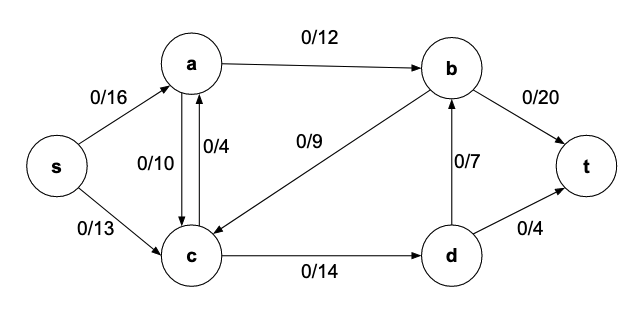
\includegraphics[width=0.75\textwidth]{4-1.png}
\end{center}

Residual Graph 1:\\
Total Flow = 12
\begin{center}
    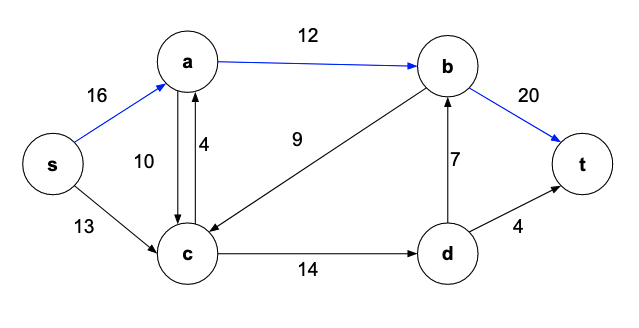
\includegraphics[width=0.75\textwidth]{4-2.png}
\end{center}

Residual Graph 2:\\
Total Flow = 12 + 4 = 16
\begin{center}
    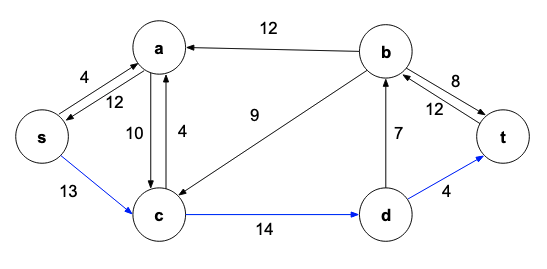
\includegraphics[width=0.75\textwidth]{4-3.png}
\end{center}

Residual Graph 3:\\
Total Flow = 16 + 7 = 23 
\begin{center}
    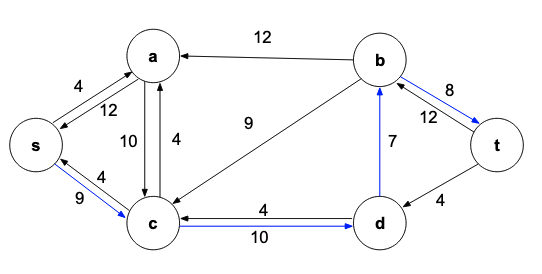
\includegraphics[width=0.75\textwidth]{4-4.png}
\end{center}

Residual Graph 4:\\
Total Flow = 23
\begin{center}
    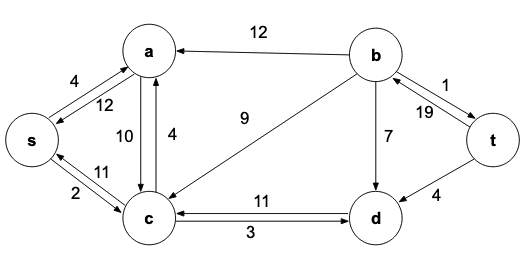
\includegraphics[width=0.75\textwidth]{4-5.png}
\end{center}

There is no augmenting in the 4th residual graph since sink vertex $t$ is not reachable from source vertex $s$. Therefore, the Edmunds-Karp algorithm is finished and we get the following graph (with flow and capacity shown) with a max flow of 23:

\begin{center}
    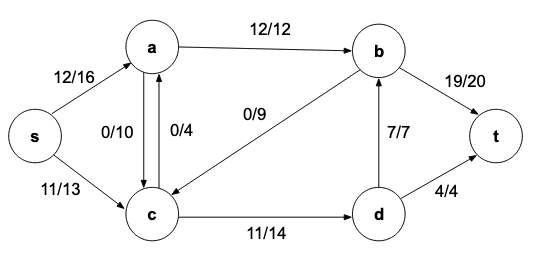
\includegraphics[width=0.75\textwidth]{4-6.png}
\end{center}

\bigskip
{\bf Question 5}\\
We want to develop an $O(m)$ algorithm that proves flow is maximal given Graph $G$ with a flow $f$ and edges stored in an adjacency list. We will return $false$ if flow is not maximal, and $true$ if flow is maximal.
\begin{lstlisting}
Create new adjacency list G'
Iterate through each vertex in G:
    G' = linked list for ever vertex in G
Iterate through the original adjacency list:
    new directed edge of vertex v to u = current flow
    new directed edge of vertex u to v = edge capacity - current flow
Breadth-First Traversal(residual graphs adjacency list):
if augmenting path is found:
    print "f is not a maxflow"
    return false
else augmenting path is not found:
    print "f is a maxflow"
    return true
\end{lstlisting}

It take $O(n)$ time to create the empty adjacency list and intialize a linked list for each vertex in the graph $G$. It take $O(m)$ time to create two edges for each edge in the residual graph. The Bread-First Search takes $O(n+m)$ time since each vertex is visited once and each edge twice. It takes $O(1)$ time to determine if there is an augmenting path and return the relative true or false value. We can determine the total running time as:
\begin{equation*} 
\begin{split}
O(n + m + n + m + 1)
\end{split}
\end{equation*}
A connected graph with n vertices has at least $n-1$ edges, so we can substitute $n$ for $m-1$:
\begin{equation*} 
\begin{split}
\Leftrightarrow \; & O((m-1) + m + (m-1) + m + 1)\\
\Leftrightarrow \; & O(4m-1)\\
\end{split}
\end{equation*}
Thus, the running time of this algorithm is $O(m)$.

\pagebreak
{\bf Question 6}\\
We want to create an algorithm that will determine the minimum number of edges that must be deleted such that the a graph G will become disconnected.
\begin{lstlisting}

Create a new adjacency list G'
n = 0   //Keep track of the vertices in G'
Iterate through each vertex in G:
    G' = linked list for every vertex in G
    n = n + 1

Iterate through each edge in G:
    create directed edges from u to v and and v to u in G'
    
Let f'(u,v) be the max flow value from u to v through G'
Set the edge capacities in G' = 1

Pick any vertex and set it as the source (s)
n = n - 1
From the remaining n-1 vertices pick a sink (t)
n = n - 1

Run the Edmonds-Karp maximum flow algorithm once: 
    minEdges = find the inital mincut value

Run the Edmonds-Karp maximum flow algorithm n-2 times:
    choose a sink (t) from the n-2 remaining vertices:
    remove the sink vertex from the remaining choices (n = n - 1)
    if mincutValue < edges variable:
        minEdges = mincutValue

return minEdges (the minimum number of edges required to disconnect the graph G)
\end{lstlisting}
In this algorithm we created the directed graph with n initialized linked lists and for each edge in $G$ we need to create two directed edges, so the running time is $O(n+m)$. Edmonds-Karp max flow algorithm takes $O(nm^2)$ time, and since were running it $n-1$ times, the Edmonds-Karp portion of this algorithm takes $O((n-1)nm^2)$ time. Thus the total running time can be determined as follows:
\begin{equation*} 
\begin{split}
\Leftrightarrow \; & O(n+m) + O((n-1)nm^2)\\
\Leftrightarrow \; & O(n+m+(n-1)nm^2)\\
\Leftrightarrow \; & O(n+m+n^2m^2-nm^2)\\
\end{split}
\end{equation*}
In terms of our big O anaylsis the simplified total running time is $O(n^2m^2)$.


\end{document}
